\section{Założenia prowadzonych badań}
\label{sec:assumptions}

%\subsection{Wymagania konstrukcyjne}
Źródłem wymuszeń mechanicznych są owalne ciała (bryły sztywne) o masie $m_s=0.03\div1.10 g$ poruszające się torem ruchu przedstawionym na Rys.\ref{fig:route}. Tor wykonany jest ze stalowej rury i w obszarze A (patrz: Rys.\ref{fig:route}) następuje sprężysty kontakt ze ścianą toru. Należy nadmienić, że w obszar A uderza 98\% poruszających się ciał. W odrębnych badaniach ustalono również, że prędkość ciała w momencie kontaktu wynosi $v_s=3.0\div7.0$ $\frac{m}{s}$. Wymuszenia mogą pojawiać się minmalnie w odstępach $T_{smin}=TODO$.

\begin{figure}[htbp]
\centering
%\fbox{
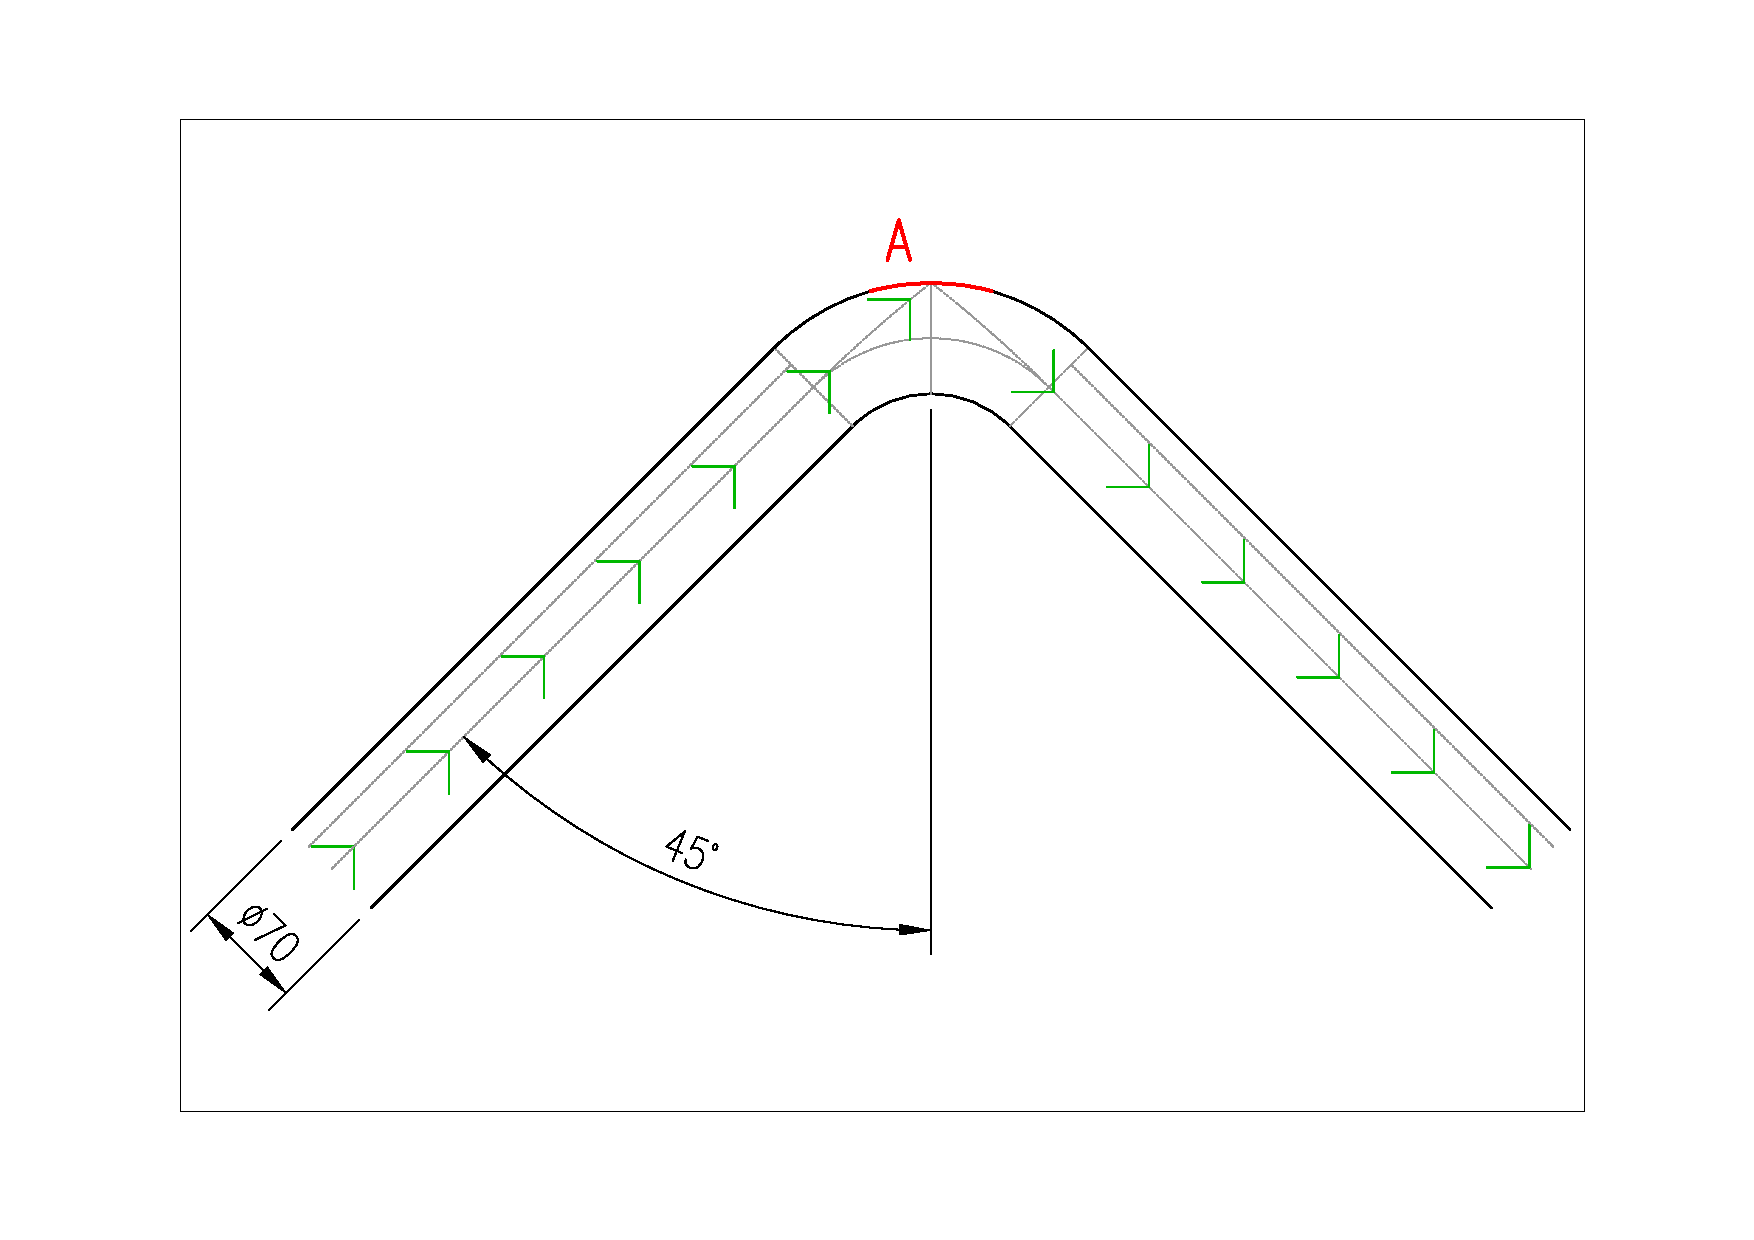
\includegraphics[width=\linewidth]{pictures/tor_lotu-dr.pdf}
%}
\caption{Zakładany tor lotu ciała fizycznego}
\label{fig:route}
\end{figure}

Założono, że miejscem montażu przetwornika jest obszar A na Rys.\ref{fig:route}, który stanowi okrąg o średnicy $d_p=TODO mm$. Dodatkowo promień ugięcia płaszczyzny A wynosi $R_A=TODOmm$, a kąt padania ciała na tę powierzchnię $\delta_p=135^{\circ}$. 

Tak ściśle i ciekawie przedstawione założenia stały się dobrym punktem wyjścia do szerzej rozumianych badań. Artykuł na naszkicowanym już przykładzie ukazuje zależność odpowiedzi elektrycznej wybranych przetworników PVDF z energią wymuszenia mechanicznego a przede wszystkim kostrukcją (zwaną także geometrią) układu.